% Fall 2021
% Source: https://eecs16b.org/student-resources/exams/fa19_final_exam.pdf

\qns{Fall 2019 Final, Question 9, Classification}

When it comes to a classification problem, we are given training data $(\vec{x_i}, \ell_i)$, where $y_i = \pm 1$, and our goal is to create a decision boundary such that most points above the boundary are '+' labeled and most points below it are '-' labeled. Formulaically: $ \vec{w}^{T} \vec{x} = 0$ is our decision boundary. Points above it satisfy $ \vec{w}^{T} \vec{x} > 0$, points below satisfy $ \vec{w}^{T} \vec{x} < 0$. 

To classify new test data, we then merely need to plug the data into the boundary equation $ \vec{w}^{T} \vec{x} $. The sign of the result, i.e.
$ sgn(\vec{w}^{T} \vec{x}) $, classifies the point as +1 if it is above the boundary ($ \vec{w}^{T} \vec{x} > 0$), and classifies it as -1 otherwise.

For example, the following data has the appropriate boundary below:

\begin{center}
    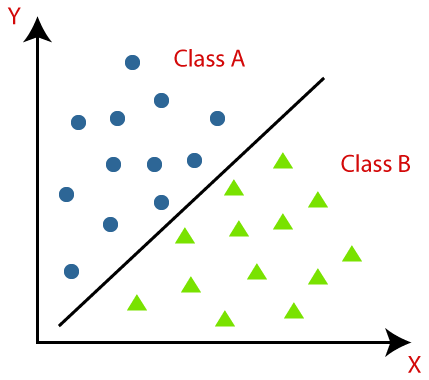
\includegraphics[scale=0.4]{\bank/ML/figures/classification-diagram.png}
\end{center}

Source: https://static.javatpoint.com/tutorial/machine-learning/images/classification-algorithm-in-machine-learning.png


Recall that we utilize a cost function that we try to minimize to get the best boundary. A least-squares cost function is inoptimal as it prioritized magnitude difference over sign, i.e. mislabeled values may not matter to it in the context of making the line as close to the data as possible.

\begin{center}
    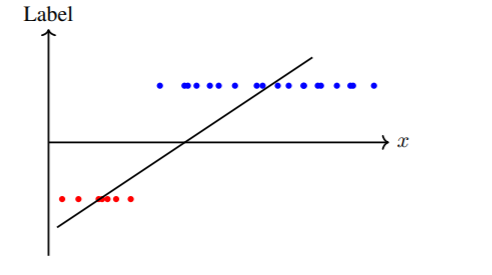
\includegraphics[scale=0.8]{\bank/ML/figures/bad_classification.PNG}
\end{center}

Source: Note 16, Classification, EECS 16B Spring 2021

Thus, we choose to customize our cost functions. We formulate the general cost function as follows:

$c_{total}(\vec{w}) = \sum_{i = 1}^{m}{c^{\ell_i}(\vec{w}^{T} \vec{x_i})}$.

Here, the idea is that for each data point, the cost function is chosen based on the label. The cost function ideally penalizes as one gets further away from the right label (i.e. going towards the wrong sign). 

Once the cost function is set up, we use Newton's Method or iterative least-squares. That is, we iteratively approximate the function as a localized quadratic around the current optimal point, then minimize that quadratic to get a new optimal point (and repeat).

We will be looking at three cost functions: Exponential, Logistic, and Quadratic. The cost functions we are considering include:

\begin{itemize}
    \item Squared loss: $c^+(p) = (p-1)^2$ and $c^-(p) = (p - (-1))^2$
    \item Exponential Loss: $c^+(p) = e^{-p}$ and $c^-(p) = c^{+p}$
    \item Logistic loss: $c^+(p) = \ln \left( 1 + e^{-p} \right)$ and $c^-(p) = \ln \left( 1 + e^{+p}\right)$
\end{itemize}

\textbf{For the plotted data, which cost functions will give reasonable answers? Select all that apply.}
\begin{center}
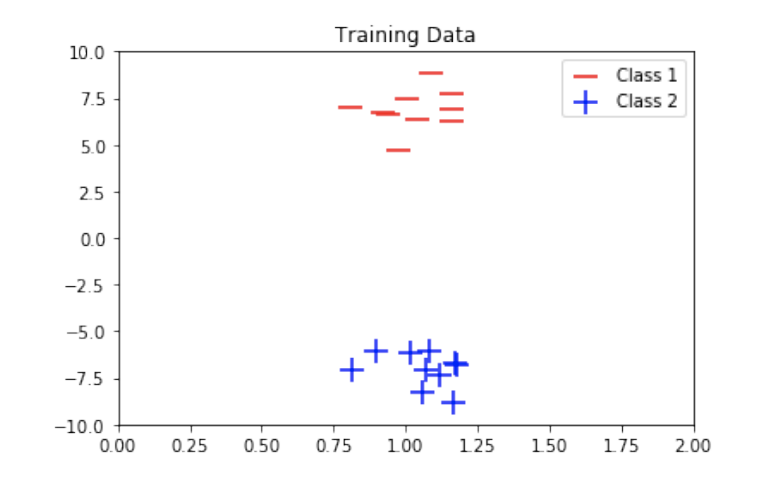
\includegraphics[width=4in, height=3in]{\bank/ML/figures/data1.png}
\begin{tabular}{| c || c | c | c |}
\hline
& \textbf{Squared} & \textbf{Exponential} & \textbf{Logistic} \\
\hline
\textbf{Reasonable Choice} & $\bigcirc$ & $\bigcirc$ & $\bigcirc$ \\
\hline
\end{tabular}
\end{center}

\sol{
This data is pretty balanced and so any of these approaches will work.
There are no outliers of any kind to confuse least-squares.
\begin{center}
\begin{tabular}{| c || c | c | c |}
\hline
& \textbf{Squared} & \textbf{Exponential} & \textbf{Logistic} \\
\hline
\textbf{Reasonable Choice} & \tikz\draw[red,fill=red] (0,0) circle (.5ex); & \tikz\draw[red,fill=red] (0,0) circle (.5ex); & \tikz\draw[red,fill=red] (0,0) circle (.5ex); \\
\hline
\end{tabular}
\end{center}
}



\begin{center}
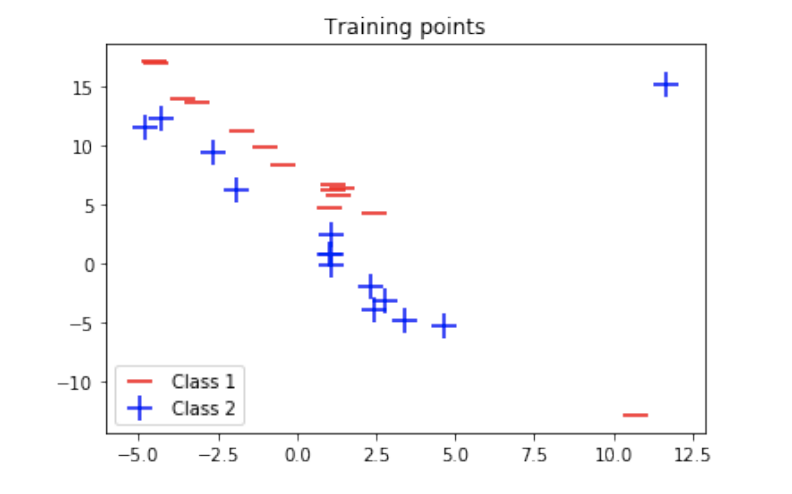
\includegraphics[width=4in, height=3in]{\bank/ML/figures/data2.png}
\begin{tabular}{| c || c | c | c |}
\hline
& \textbf{Squared} & \textbf{Exponential} & \textbf{Logistic} \\
\hline
\textbf{Reasonable Choice} & $\bigcirc$ & $\bigcirc$ & $\bigcirc$ \\
\hline
\end{tabular}
\end{center}

\sol{
This data clearly has a ``wrongly classified'' outlier that is a ``+'' point deep in what should be ``-'' territory.
Both the squared loss and (especially) exponential loss will be quite sensitive to this while logistic loss will end up largely ignoring this point.
In such cases, we really need to be using logistic loss of the choices
offered here.
\begin{center}
\begin{tabular}{| c || c | c | c |}
\hline
& \textbf{Squared} & \textbf{Exponential} & \textbf{Logistic} \\
\hline
\textbf{Reasonable Choice} & $\bigcirc$ & $\bigcirc$ & \tikz\draw[red,fill=red] (0,0) circle (.5ex); \\
\hline
\end{tabular}
\end{center}
}

\begin{center}
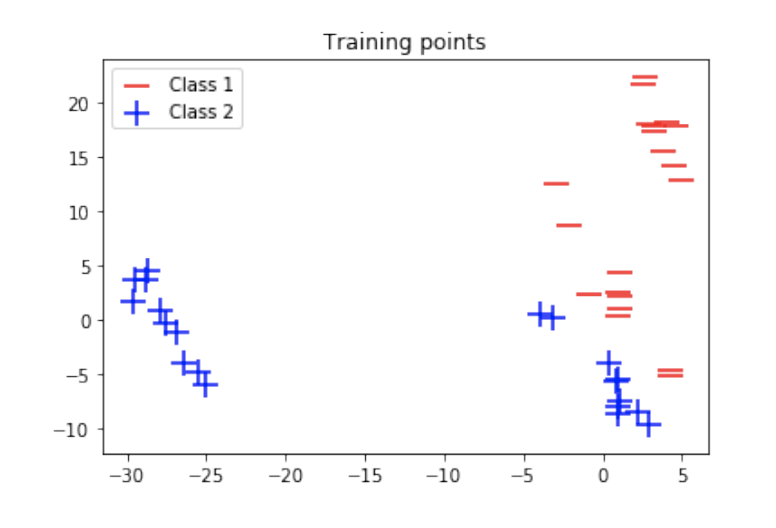
\includegraphics[width=4in, height=3in]{\bank/ML/figures/data3.png}
\begin{tabular}{| c || c | c | c |}
\hline
& \textbf{Squared} & \textbf{Exponential} & \textbf{Logistic} \\
\hline
\textbf{Reasonable Choice} & $\bigcirc$ & $\bigcirc$ & $\bigcirc$ \\
\hline
\end{tabular}
\end{center}

\sol{
In this case, we clearly have two masses of points in each category.
The + category is particularly striking because the second mass of points is deep within what we would consider ``+'' category.
These type of points will confuse squared loss quite a bit while both exponential and logistic loss don’t care about points that are deeply within their own proper territories.
They focus on things closer to the boundaries.
\begin{center}
\begin{tabular}{| c || c | c | c |}
\hline
& \textbf{Squared} & \textbf{Exponential} & \textbf{Logistic} \\
\hline
\textbf{Reasonable Choice} & $\bigcirc$ & \tikz\draw[red,fill=red] (0,0) circle (.5ex); & \tikz\draw[red,fill=red] (0,0) circle (.5ex); \\
\hline
\end{tabular}
\end{center}
}


\begin{center}
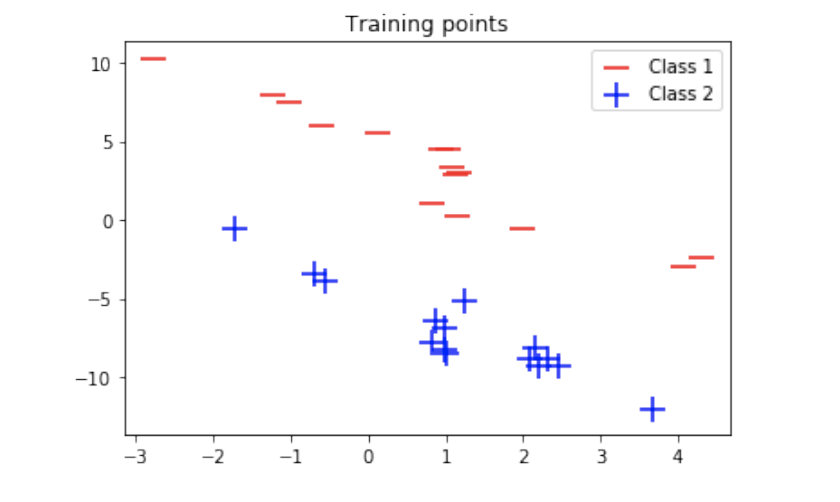
\includegraphics[width=4in, height=3in]{\bank/ML/figures/data4.png}
\begin{tabular}{| c || c | c | c |}
\hline
& \textbf{Squared} & \textbf{Exponential} & \textbf{Logistic} \\
\hline
\textbf{Reasonable Choice} & $\bigcirc$ & $\bigcirc$ & $\bigcirc$ \\
\hline
\end{tabular}
\end{center}

\sol{
This is actually an example with thin parallel categories that have no outliers.
For this kind of data, even squared-loss will work fine because of the balanced nature of the training data.
However, in this kind of example, because the mass distribution doesn’t necessarily reflect the parallel structure of the true boundary, mean-based classification won’t work as well.
However, that is not a choice that you are offered here.
\begin{center}
\begin{tabular}{| c || c | c | c |}
\hline
& \textbf{Squared} & \textbf{Exponential} & \textbf{Logistic} \\
\hline
\textbf{Reasonable Choice} & \tikz\draw[red,fill=red] (0,0) circle (.5ex); & \tikz\draw[red,fill=red] (0,0) circle (.5ex); & \tikz\draw[red,fill=red] (0,0) circle (.5ex); \\
\hline
\end{tabular}
\end{center}
}